\RequirePackage{plautopatch}
\documentclass[platex,dvipdfmx,a4paper]{jsarticle}

\usepackage{amsmath}
\usepackage{amsfonts}
\usepackage{amssymb}

\usepackage[dvipdfmx]{graphicx}
\usepackage{float}

\usepackage{tikz}
\usepackage{caption}

% 「%」は以降の内容を「改行コードも含めて」無視するコマンド
\usepackage[%
  dvipdfmx,% 欧文ではコメントアウトする
  setpagesize=false,%
  bookmarks=true,%
  bookmarksdepth=tocdepth,%
  bookmarksnumbered=true,%
  colorlinks=false,%
  pdftitle={},%
  pdfsubject={},%
  pdfauthor={},%
  pdfkeywords={}%
]{hyperref}
% PDFのしおり機能の日本語文字化けを防ぐ((u)pLaTeXのときのみかく)
\usepackage{pxjahyper}

\usepackage{framed}
\setlength{\OuterFrameSep}{0pt}

\usepackage{physics2}
\usephysicsmodule{ab}
\usephysicsmodule{ab.braket}


\newcommand{\hb}[2]{\frac{\partial #1}{\partial #2}}
\newcommand{\bbn}[2]{\frac{d #1}{d #2}}
\newcommand{\nhb}[3]{\frac{\partial^{#1} #2}{\partial #3^{#1}}}
\newcommand{\nbbn}[3]{\frac{d^{#1} #2}{d #3^{#1}}}
\newcommand{\vectxy}[2]{\begin{bmatrix}#1\\#2\end{bmatrix}}
\newcommand{\vectxyz}[3]{\begin{bmatrix}#1\\#2\\#3\end{bmatrix}}
\newcommand{\vect}[1]{\boldsymbol{\mathrm{#1}}}

\newcommand{\ssum}[3]{\sum_{#1=#2}^#3}

\newcommand{\veff}{V_{\mathrm{eff}}(r)}

\hypersetup{colorlinks=true}
\hypersetup{linkcolor=red}

\title{量子力学入門演習レポート4}
\author{25B00729　嶋田 悠音}

\begin{document}
\maketitle
\subsection*{(1)}

ポテンシャル $V(x)$ が $x=a$ において不連続である場合を考える。ただし，ポテンシャルは有限であると仮定する。このとき，定常状態の波動関数 $\psi_E(x)$ およびその一階微分に対する境界条件を，定常状態に対する Schr\"odinger 方程式から導出する。

定常状態の Schr\"odinger 方程式は

\begin{align*}
-\frac{\hbar^2}{2m}\nhb{2}{\psi_E}{x}
+V(x)\psi_E(x)
=
E\psi_E(x)
\end{align*}

で与えられる。

まず，この式を区間 $[a-\varepsilon,a+\varepsilon]$ で積分する：

\begin{align*}
-\frac{\hbar^2}{2m}
\int_{a-\varepsilon}^{a+\varepsilon}
\psi_E''(x)\,dx
+
\int_{a-\varepsilon}^{a+\varepsilon}
(V(x)-E)\psi_E(x)\,dx
=
0。
\end{align*}

第一項を積分すると，

\begin{align*}
-\frac{\hbar^2}{2m}
\left[
\psi_E'(x)
\right]_{a-\varepsilon}^{a+\varepsilon}
+
\int_{a-\varepsilon}^{a+\varepsilon}
(V(x)-E)\psi_E(x)\,dx
=
0
\end{align*}

を得る。

ここで，ポテンシャル $V(x)$ は有限であり，波動関数 $\psi_E(x)$ も有限であるから，被積分関数
$(V(x)-E)\psi_E(x)$
は有限。したがって，

\begin{align*}
\lim_{\varepsilon\to0}
\int_{a-\varepsilon}^{a+\varepsilon}
(V(x)-E)\psi_E(x)\,dx
=
0
\end{align*}

が成り立つ。

よって，上式の $\varepsilon\to0$ 極限を取ると，

\begin{align*}
-\frac{\hbar^2}{2m}
\lim_{\varepsilon\to0}
\left[
\psi_E'(a+\varepsilon)
-\psi_E'(a-\varepsilon)
\right]
=
0
\end{align*}

となる。したがって，

\begin{align*}
\psi_E'(a+0)
=
\psi_E'(a-0)
\end{align*}

を得る。

また，波動関数自身も連続であるため、
\begin{align*}
\psi_E(a+0)
=
\psi_E(a-0)
\end{align*}

が成り立つ。

以上より，有限の不連続ポテンシャルに対して定常状態の波動関数が満たす境界条件は

\begin{align*}
\psi_E(a+0)
&=
\psi_E(a-0),\\
\psi_E'(a+0)
&=
\psi_E'(a-0)
\end{align*}

である。

\subsection*{(2)}

ポテンシャル

\begin{align*}
V(x)
=
\begin{cases}
0 &( |x|\le L),\\
\infty &( |x|>L)
\end{cases}
\end{align*}

を考える。

外側では粒子は存在できないため，

\begin{align*}
\psi_E(x)=0
\qquad
(|x|>L)
\end{align*}

である。また，波動関数の連続性より，

\begin{align*}
\psi_E(-L)=\psi_E(L)=0
\end{align*}

が境界条件となる。

井戸の内部 $|x|<L$ では $V(x)=0$ であるから，定常状態に対する Schr\"odinger 方程式は

\begin{align*}
-\frac{\hbar^2}{2m}\nhb{2}{\psi_E}{x}
=
E\psi_E
\end{align*}

となる。

まず，$E\le0$ の場合を考える。$E=0$ のとき一般解は

\begin{align*}
\psi_E(x)=Ax+B
\end{align*}

であるが，境界条件を課すと $A=B=0$ しか得られない。

また，$E<0$ の場合には一般解は双曲線関数で与えられるが，境界条件を課すとやはり自明解しか存在しない。

したがって，非自明な解が存在するためには

\begin{align*}
E>0
\end{align*}

でなければならない。

ここで，

\begin{align*}
k=\frac{\sqrt{2mE}}{\hbar}
\end{align*}

とおくと，Schr\"odinger 方程式は

\begin{align*}
\nhb{2}{\psi_E}{x}+k^2\psi_E=0
\end{align*}

となる。

その一般解は

\begin{align*}
\psi_E(x)
=
A\cos(kx)
+
B\sin(kx)
\end{align*}

である。

境界条件 $\psi_E(\pm L)=0$ を課すと，

\begin{align*}
A\cos(kL)+B\sin(kL)&=0,\\
A\cos(kL)-B\sin(kL)&=0
\end{align*}

を得る。

両式を加減することにより，

\begin{align*}
A\cos(kL)&=0,\\
B\sin(kL)&=0
\end{align*}

となる。

非自明な解が存在するためには，

\begin{align*}
kL=\frac{n\pi}{2}
\qquad
(n=1,2,3,\cdots)
\end{align*}

でなければならない。

したがって，許される波数は

\begin{align*}
k_n
=
\frac{n\pi}{2L}
\qquad
(n=1,2,3,\cdots)
\end{align*}

であり，エネルギー固有値は

\begin{align*}
E_n
&=
\frac{\hbar^2k_n^2}{2m}\\
&=
\frac{\hbar^2\pi^2}{8mL^2}n^2
\qquad
(n=1,2,3,\cdots)
\end{align*}

となる。

対応する固有関数は

\begin{align*}
\psi_n(x)
=
\begin{cases}
\displaystyle
\frac{1}{\sqrt L}
\sin\left(
\frac{n\pi(x+L)}{2L}
\right)
&( |x|\le L),\\
0&( |x|>L)
\end{cases}
\end{align*}

である。

エネルギーの低い方から4つの状態は

\begin{align*}
\psi_1(x)
&=
\frac{1}{\sqrt L}
\cos\left(
\frac{\pi x}{2L}
\right),\\
\psi_2(x)
&=
\frac{1}{\sqrt L}
\sin\left(
\frac{\pi x}{L}
\right),\\
\psi_3(x)
&=
\frac{1}{\sqrt L}
\cos\left(
\frac{3\pi x}{2L}
\right),\\
\psi_4(x)
&=
\frac{1}{\sqrt L}
\sin\left(
\frac{2\pi x}{L}
\right)
\end{align*}

であり，対応するエネルギーは

\begin{align*}
E_n
=
\frac{\hbar^2\pi^2}{8mL^2}n^2
\qquad
(n=1,2,3,4)
\end{align*}

である。

\subsection*{(3)}

ポテンシャル

\begin{align*}
V(x)
=
\begin{cases}
\infty &(x<0),\\
-V_0 &(0\le x\le L),\\
0 &(x>L)
\end{cases}
\qquad
(V_0>0)
\end{align*}

を考える。

束縛状態では

\begin{align*}
-V_0<E<0
\end{align*}

が成り立つ。

領域ごとに Schr\"odinger 方程式を解く。

まず，領域 $0\le x\le L$ ではポテンシャルは一定値 $-V_0$ であるから，

\begin{align*}
-\frac{\hbar^2}{2m}
\nhb{2}{\psi}{x}
-V_0\psi
=
E\psi
\end{align*}

となる。

ここで

\begin{align*}
k
=
\frac{\sqrt{2m(E+V_0)}}{\hbar}
\end{align*}

とおけば，

\begin{align*}
\nhb{2}{\psi}{x}
+k^2\psi
=
0
\end{align*}

を得る。

したがって，一般解は

\begin{align*}
\psi_{\mathrm I}(x)
=
A\sin(kx)
+
B\cos(kx)
\end{align*}

である。

一方，$x=0$ には無限壁が存在するため，

\begin{align*}
\psi(0)=0
\end{align*}

でなければならない。

よって，

\begin{align*}
B=0
\end{align*}

であり，

\begin{align*}
\psi_{\mathrm I}(x)
=
A\sin(kx)
\end{align*}

となる。

次に，領域 $x>L$ ではポテンシャルは零であるから，

\begin{align*}
-\frac{\hbar^2}{2m}
\nhb{2}{\psi}{x}
=
E\psi
\end{align*}

となる。

束縛状態では $E<0$ であるため，

\begin{align*}
\kappa
=
\frac{\sqrt{-2mE}}{\hbar}
\end{align*}

とおくと，

\begin{align*}
\nhb{2}{\psi}{x}
-\kappa^2\psi
=
0
\end{align*}

を得る。

一般解は

\begin{align*}
\psi_{\mathrm{II}}(x)
=
Ce^{\kappa x}
+
De^{-\kappa x}
\end{align*}

である。

しかし束縛状態では

\begin{align*}
\lim_{x\to\infty}\psi(x)=0
\end{align*}

でなければならないので，

\begin{align*}
C=0
\end{align*}

である。

したがって，

\begin{align*}
\psi_{\mathrm{II}}(x)
=
De^{-\kappa x}
\end{align*}

となる。

次に，$x=L$ において波動関数とその一階微分の連続性を課す。

まず波動関数の連続性より，

\begin{align*}
A\sin(kL)
=
De^{-\kappa L}
\end{align*}

を得る。

また，一階微分の連続性より，

\begin{align*}
Ak\cos(kL)
=
-\kappa De^{-\kappa L}
\end{align*}

が成り立つ。

第1式で第2式を割ることにより，

\begin{align*}
k\cot(kL)
=
-\kappa
\end{align*}

を得る。

ここで，

\begin{align*}
k
=
\frac{\sqrt{2m(E+V_0)}}{\hbar},
\qquad
\kappa
=
\frac{\sqrt{-2mE}}{\hbar}
\end{align*}

を代入すると，

\begin{align*}
\frac{\sqrt{2m(E+V_0)}}{\hbar}
\cot\left(
\frac{\sqrt{2m(E+V_0)}}{\hbar}L
\right)
=
-\frac{\sqrt{-2mE}}{\hbar}
\end{align*}

となる。

両辺に $\hbar$ を掛ければ，

\begin{align*}
\sqrt{2m(E+V_0)}
\cot\left(
\frac{\sqrt{2m(E+V_0)}}{\hbar}L
\right)
=
-\sqrt{-2mE}
\end{align*}

を得る。

以上より，束縛状態の固有エネルギーは，超越方程式

\begin{align*}
\sqrt{2m(E+V_0)}
\cot\left(
\frac{\sqrt{2m(E+V_0)}}{\hbar}L
\right)
=
-\sqrt{-2mE}
\end{align*}

の解として定まる。

\subsection*{(4)}

(3) で得られた束縛状態の条件式

\begin{align*}
k\cot(kL)
=
-\kappa
\end{align*}

を無次元量

\begin{align*}
\xi
=
kL,
\qquad
\eta
=
\kappa L
\end{align*}

を用いて書き直す。

まず，束縛状態の条件式は

\begin{align*}
\xi\cot\xi
=
-\eta
\end{align*}

となる。したがって，

\begin{align*}
\eta
=
-\xi\cot\xi
\end{align*}

で表される曲線を考えればよい。

次に，

\begin{align*}
\xi
=
\frac{\sqrt{2m(E+V_0)}}{\hbar}L,
\qquad
\eta
=
\frac{\sqrt{-2mE}}{\hbar}L
\end{align*}

の両辺を二乗すると，

\begin{align*}
\xi^2
&=
\frac{2m(E+V_0)L^2}{\hbar^2},\\
\eta^2
&=
\frac{-2mEL^2}{\hbar^2}
\end{align*}

を得る。

これらを加えると，

\begin{align*}
\xi^2+\eta^2
=
\frac{2mV_0L^2}{\hbar^2}
\end{align*}

となる。

ここで

\begin{align*}
R
=
\frac{\sqrt{2mV_0}}{\hbar}L
\end{align*}

とおけば，

\begin{align*}
\xi^2+\eta^2
=
R^2
\end{align*}

となるので，$(\xi,\eta)$ 平面では原点を中心とする半径 $R$ の円を表す。

したがって，束縛状態は

\begin{align*}
\eta=-\xi\cot\xi
\end{align*}

で与えられる曲線と，

\begin{align*}
\xi^2+\eta^2=R^2
\end{align*}

で与えられる上半円との交点として求められる。

\begin{center}
  \begin{minipage}{0.75\textwidth}
    \centering
    \begin{tikzpicture}[scale=1.1]

      \draw[->] (0,0) -- (6.5,0) node[right] {$\xi$};
      \draw[->] (0,0) -- (0,4.5) node[above] {$\eta$};

      \draw[domain=1.58:3.10,smooth,samples=200]
        plot({\x},{-(\x)*(cos(\x r)/sin(\x r))});

      \draw[domain=4.72:6.25,smooth,samples=200]
        plot({\x},{-(\x)*(cos(\x r)/sin(\x r))});

      \draw[thick]
        plot[domain=0:5,samples=200]
        ({\x},{sqrt(25-\x*\x)});

      \draw[dashed] ({pi/2},0) -- ({pi/2},4.0);
      \node[below] at ({pi/2},0) {$\pi/2$};

      \node at (4.1,3.1)
        {$\xi^2+\eta^2=R^2$};

      \node at (2.5,0.9)
        {$\eta=-\xi\cot\xi$};

    \end{tikzpicture}
    \captionof*{figure}{$\eta=-\xi\cot\xi$ と上半円 $\xi^2+\eta^2=R^2$ の交点が束縛状態を与える。}
  \end{minipage}
\end{center}

束縛状態の個数は，半径 $R$ の上半円と曲線 $\eta=-\xi\cot\xi$ の交点の個数に等しい。

また，$\eta=-\xi\cot\xi$ は

\begin{align*}
\frac{\pi}{2}
<
\xi
<
\pi,
\qquad
\frac{3\pi}{2}
<
\xi
<
2\pi,
\qquad \cdots
\end{align*}

の各区間で正の値を取る。

したがって，半径 $R$ を大きくすると交点の数が増加し，それに応じて束縛状態の数も増加する。

以上より，束縛状態は

\begin{align*}
\eta=-\xi\cot\xi,
\qquad
\xi^2+\eta^2
=
\frac{2mV_0L^2}{\hbar^2}
\end{align*}

の交点として幾何学的に求められる。
\end{document}